\section{Características}

\begin{frame}\frametitle{Extracción de características}
  \begin{itemize}
  \item Las \textit{características} (\textit{features}) son conjuntos de valores derivados de una señal o de un conjunto de mediciones, que permiten describir el conjunto original y que son informativos y no redundantes.
  \item   Unas de las características más simples que se pueden extraer de una imagen son líneas y otras formas geométricas simples.
  \item El vector de características que describe una línea puede ser el conjunto de parámetros de su ecuación.
  \item Los vectores de características también se pueden utilizar para reconocer objetos, usando características cmo color, tamaño, forma, volumen, entre otras.
   \item Más adelante se verá la Transformada SIFT, uno de los algoritmos más usados para extracción de características. 
  \end{itemize}
\end{frame}

\begin{frame}\frametitle{La Transformada Hough}
  La Transformada Hough es un método que permite encontrar líneas, círculos y otras formas geométricas que se puedan describir fácilmente mediante expresiones analíticas. En el caso de las líneas, se trata de encontrar los dos parámetros que describen la recta:
  \begin{columns}
    \begin{column}{0.4\textwidth}
      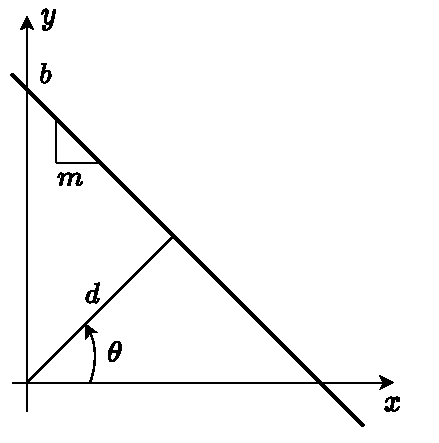
\includegraphics[width=\textwidth]{Figures/Hough2.pdf}
    \end{column}
    \begin{column}{0.6\textwidth}
      \begin{itemize}
      \item La forma pendiente-ordenada $y = mx + b$ tiene la desventaja de no poder expresar líneas verticales.
      \item La forma canónica $Ax + By + C$ requiere de una normalización $A_1 x + B_1 y + 1 = 0$ para que solo sean dos parámetros.
      \item Una forma más conveniente, es la forma normal $d = x\cos\theta + y\sin\theta$
      \item Esta última forma tiene una ventaja: si la línea correponde a un borde, el ángulo $\theta$ será la dirección del gradiente. 
      \end{itemize}
    \end{column}
  \end{columns}
\end{frame}

\begin{frame}\frametitle{El Espacio de Hough}
  El Espacio de Hough, para el caso de las líneas, es el conjunto de todos los posibles pares $(\theta, d)$.
  \begin{itemize}
  \item Una recta $L$ en el espacio cartesiano corresponde a un punto $P_h$ en el Espacio de Hough
  \item Un punto $P_c$ en el espacio cartesiano corresponde a una curva $C$ en el Espacio de Hough. Esta curva representa los parámetros $(\theta_i, d_i)$ de todas las rectas $L_i$ que pasan por el punto $P$.
  \end{itemize}
  \begin{figure}
    \centering
    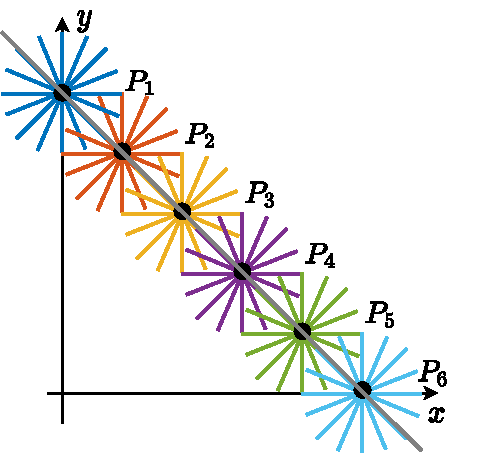
\includegraphics[width=0.35\textwidth]{Figures/Hough1.pdf}
    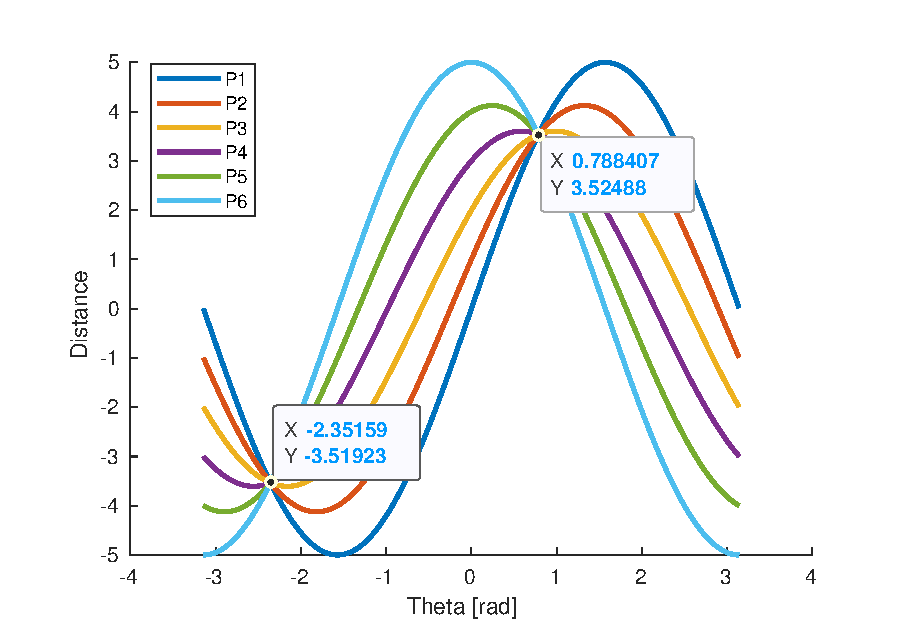
\includegraphics[width=0.5\textwidth]{Figures/Hough1.eps}
  \end{figure}
\end{frame}

\begin{frame}\frametitle{Extracción de Líneas por Transformada Hough}
  Este método consiste en encontrar las curvas $C_i$ en el espacio de Hough que pasan por cada punto $P_c$ en el espacio cartesiano. Los puntos $P_h$ en el Espacio de Hough por donde pasen más curvas $C_i$ corresponderán a las rectas resultantes en el espacio cartesiano.
  \begin{figure}
    \centering
    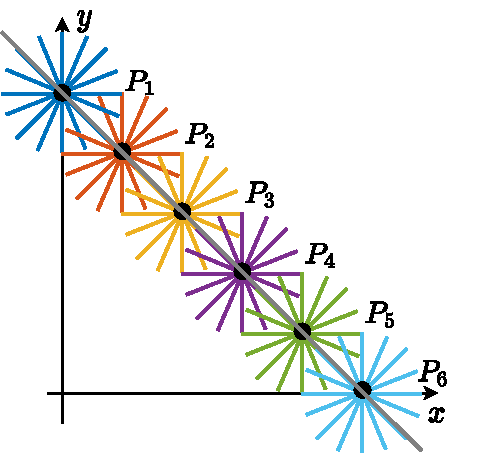
\includegraphics[width=0.35\textwidth]{Figures/Hough1.pdf}
    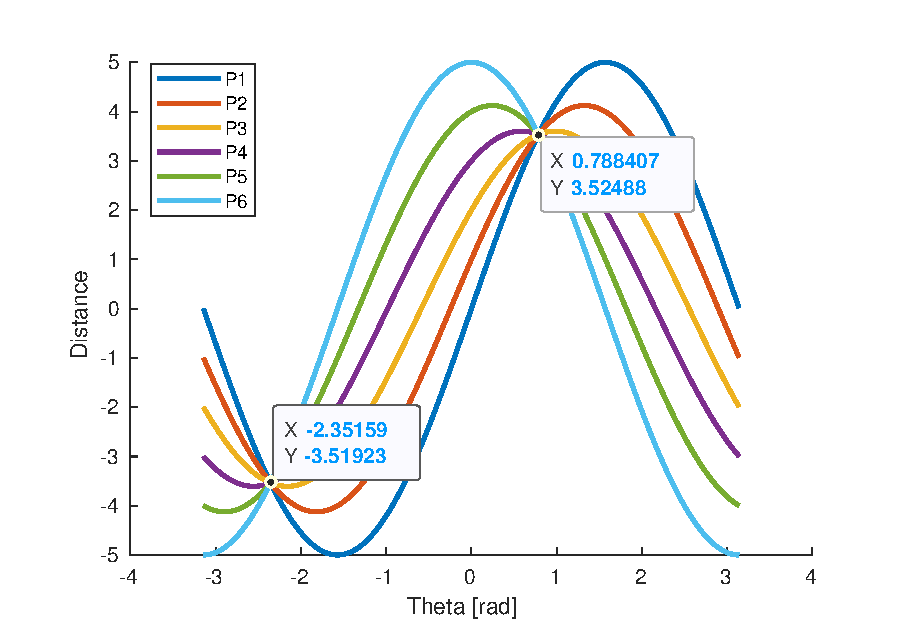
\includegraphics[width=0.5\textwidth]{Figures/Hough1.eps}
  \end{figure}
\end{frame}

\begin{frame}\frametitle{Extracción de Líneas por Transformada Hough}
  \begin{algorithm}[H]
    \KwIn{Imagen binaria $M$, umbral mínimo de votos $a_{min}$}
    \KwOut{Líneas expresadas en la forma $(d,\theta)$}
    \DontPrintSemicolon
    \;
    Inicializar en 0 un conjunto $A$ de acumuladores para cada par cuantizado $(d_k,\theta_k)$\;
    \ForAll{Pixel $M[i,j] \neq 0$}
    {
      \ForAll{Ángulo $\theta_k$ cuantizdo}
      {
        $d = j\cos\theta_k + i\sin\theta_k$
        $d_k = $ valor cuantizado de $d$
        Incrementar en uno el acumulador correspondiente $A[d_k, \theta_k]$
      }
    }
    \ForAll{$a \in A$}
    {
      \If{$a > a_{min}$}
      {
        Agregar la línea $(d_k, \theta_k)$ al conjunto de líneas detectadas
      }
    }
    Devolver el conjunto de líneas detectadas
  \end{algorithm}
\end{frame}

\begin{frame}\frametitle{Extracción de círculos por T. Hough}
  De la ecuación de un círculo en el plano:
  \[(x - c_x)^2 + (y - c_y)^2 = r^2\]
  Se puede observar que un círculo está definido por tres parámetros $(c_x, c_y, r)$.
  \begin{itemize}
  \item De forma similar a las líneas, se podrían fijar dos parámetros y calcular el tercero
  \item Sin embargo variar dos parámetros incrementa la complejidad considerablemente
  \item Se puede utilizar el ángulo del gradiente y un variar el valor del radio $r$ para determinar el centro, de este modo, solo se tiene que variar un parámetro.
  \item Se considera que el gradiente apunta hacia el centro del círculo. 
  \end{itemize}
\end{frame}

\begin{frame}\frametitle{T. Hough Generalizada}
  Hasta el momento la T. Hough se ha usado para detectar formas determinadas analíticamente. Se pueden detectar formas arbitrarias si se dispone de una descripción de la forma a detectar y, al igual que con círculos y líneas, se varían los parámetros y se hace un sistema de votos.
  \begin{itemize}
  \item La descripción de la forma se hace mediante la llamada \textit{Tabla R}
  \item Los parámetros que se pueden variar son el centro $(x_c, y_c)$, la rotación $\theta$ y la escala $(S_x, S_y)$
  \end{itemize}
  
\end{frame}

\begin{frame}\frametitle{T. H. Generalizada - Tabla R}
  La Tabla R es una descripción de la figura en función del ángulo del gradiente.
  \begin{figure}
    \centering
    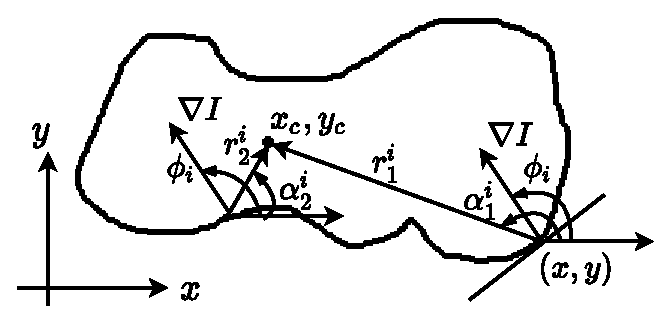
\includegraphics[width=0.5\textwidth]{Figures/HoughTableR.pdf}
  \end{figure}
  \begin{itemize}
  \item Se selecciona un centro arbitrario $(x_c, y_c)$
  \item Para cada punto $(x,y)$ en la figura, se calcula el ángulo del gradiente y se cuantiza a un ángulo $\phi_i$. 
  \item Para el mismo punto, se calcula el vector del punto al centro $(x_c - x, y_c - y)$ que se puede expresar en la forma polar $(r,\alpha)$
  \item A cada ángulo cuantizado $\phi_i$ se le pueden asociar varios valores $(r_1^i, \alpha_1^i),\dots , (r_j^i, \alpha_j^i)$
  \end{itemize}
\end{frame}

\begin{frame}\frametitle{T. H. Generalizada - Tabla R}
  Con la información anterior se construye la Tabla R:
  \[\]
  \begin{table}
    \centering
  \begin{tabular}{l|l}
    Ángulo del Gradiente & Vector al centro \\
    \hline
    $\phi_1$ & $(r_1^1, \alpha_1^1),\dots , (r_j^1, \alpha_j^1)$\\
    $\phi_2$ & $(r_1^2, \alpha_1^2),\dots , (r_j^2, \alpha_j^2)$\\
    $\vdots$ & $\vdots$\\
    $\phi_i$ & $(r_1^i, \alpha_1^i),\dots , (r_j^i, \alpha_j^i)$\\
    $\vdots$ & $\vdots$\\
    $\phi_n$ & $(r_1^n, \alpha_1^n),\dots , (r_j^n, \alpha_j^n)$
  \end{tabular}
  \end{table}
  \[\]
  La Tabla R funciona como una descripción de la forma arbitraria.
\end{frame}

\begin{frame}\frametitle{Detección de formas generales}
  El caso más sencillo se da cuando se tiene una forma en la imagen del mismo tamaño y orientación que el patrón original. En este caso solo es necesario determinar el centro, por lo que el Espacio de Hough solo tiene dos dimensiones: los parámetros $x_c, y_c$.
  \begin{algorithm}[H]
    \small
    \KwIn{Imagen binaria $M$, umbral mínimo de votos $a_{min}$}
    \KwOut{Formas generales definidas por la tabla R con centro en $(x_c,y_c)$}
    \DontPrintSemicolon
    \;
    Inicializar en 0 un conjunto $A$ de acumuladores para cada par cuantizado $(x_c,y_c)$\;
    \ForAll{Pixel $M[x,y] \neq 0$}
    {
      Determinar el ángulo $\phi$ del gradiente en el punto $x,y$ y cuantizarlo a un valor $\phi_i$\;
      \ForAll{Vector $(r_i^j, \alpha_i^j)$ asociado al ángulo $\phi_i$ en la Tabla R}
      {
        Determinar las coordenadas del centro:\;
        $x_c^j = x + \cos\alpha_i^j$\;
        $y_c^j = y + \sin\alpha_i^j$
        Incrementar en uno el acumulador correspondiente $A[x_c^j, y_c^j]$
      }
    }
    \ForAll{$a \in A$}
    {
      \If{$a > a_{min}$}
      {
        Agregar el patrón con centro en $(x_c, y_c)$ al conjunto de patrones detectados
      }
    }
    Devolver el conjunto de patrones detectados
  \end{algorithm}  
\end{frame}

\begin{frame}\frametitle{Detección de formas generales}
  Para detectar patrones con orientación $\theta$ y escala $S$ arbitrarios, se aplica el mismo principio, pero con un espacio de Hough de cuatro dimensiones: $(x_c, y_c, \theta, S$
  \begin{algorithm}[H]
    \small
    \KwIn{Imagen binaria $M$, umbral mínimo de votos $a_{min}$ }
    \KwOut{Formas generales definidas por la tabla $R$}
    \DontPrintSemicolon
    \;
    Inicializar en 0 un conjunto $A$ de acumuladores para cada tupla cuantizada $(x_c,y_c,\theta, S)$\;
    \ForAll{Pixel $M[x,y] \neq 0$}
    {
      Determinar el ángulo $\phi$ del gradiente en el punto $x,y$ y cuantizarlo a un valor $\phi_i$\;
      \ForAll{Orientación cuantizada $\theta$}
      {
        \ForAll{Escala cuantizada $S$}
        {
          \ForAll{Vector $(r_i^j, \alpha_i^j)$ asociado al ángulo $\phi_i$ en la Tabla R}
          {
            Determinar las coordenadas del centro:\;
            $x_c^j = x + S\cos(\alpha_i^j + \theta)$\;
            $y_c^j = y + S\sin(\alpha_i^j + \theta)$\;
            Incrementar en uno el acumulador correspondiente $A[x_c^j, y_c^j, \theta, S]$
          }
        }
      }
    }
    Devolver el conjunto de patrones donde el acumulador $A[x_c^j, y_c^j, \theta, S] > a_{min}$
  \end{algorithm}  
\end{frame}

\begin{frame}\frametitle{Detección de esquinas}
  Una esquina se puede considerar como un punto donde, en una vecindad $W$, el gradiente tiene dos direcciones dominantes diferentes.
  \begin{itemize}
  \item Aunque las esquinas representan un porcentaje muy pequeño de la imagen, suelen ser puntos de mucho interés.
  \item Las esquinas se consideran puntos de interés invariantes a escala, rotación e iluminación
  \item Entre algunas aplicaciones se encuentran:
    \begin{itemize}
    \item Registro de imágenes
    \item Reconstrucción de escenas 3D
    \item Detección de movimiento
    \item Reconocimiento de objetos
    \end{itemize}
  \end{itemize}
\end{frame}

\begin{frame}\frametitle{Detector de esquinas de Harris}
  Este detector se basa en la autocorrelación de los valores del gradiente en una vencidad de un pixel $(x,y)$. La detección se puede sintetizar en los siguientes pasos:
  \begin{itemize}
  \item Obtención de las derivadas parciales
  \item Obtención de la matriz del segundo momento
  \item Cálculo de la respuesta de Harris
  \item Supresión de no máximos
  \end{itemize}
\end{frame}

\begin{frame}\frametitle{Laplaciano de Gaussiano (LoG)}
  El Laplaciano de una función está definido como:
  \[\nabla^2 I = \frac{\partial^2 I}{\partial x^2} + \frac{\partial^2 I}{\partial y^2}\]
  Aplicando diferencias finitas, el Laplaciano se puede aproximar con el Kernel:
  \[\left[\begin{tabular}{ccc}0 & 1 & 0\\1 & -4 & 1\\0 & 1 & 0\end{tabular}\right]\]
\end{frame}
